\documentclass[1p]{elsarticle_modified}
%\bibliographystyle{elsarticle-num}

%\usepackage[colorlinks]{hyperref}
%\usepackage{abbrmath_seonhwa} %\Abb, \Ascr, \Acal ,\Abf, \Afrak
\usepackage{amsfonts}
\usepackage{amssymb}
\usepackage{amsmath}
\usepackage{amsthm}
\usepackage{scalefnt}
\usepackage{amsbsy}
\usepackage{kotex}
\usepackage{caption}
\usepackage{subfig}
\usepackage{color}
\usepackage{graphicx}
\usepackage{xcolor} %% white, black, red, green, blue, cyan, magenta, yellow
\usepackage{float}
\usepackage{setspace}
\usepackage{hyperref}

\usepackage{tikz}
\usetikzlibrary{arrows}

\usepackage{multirow}
\usepackage{array} % fixed length table
\usepackage{hhline}

%%%%%%%%%%%%%%%%%%%%%
\makeatletter
\renewcommand*\env@matrix[1][\arraystretch]{%
	\edef\arraystretch{#1}%
	\hskip -\arraycolsep
	\let\@ifnextchar\new@ifnextchar
	\array{*\c@MaxMatrixCols c}}
\makeatother %https://tex.stackexchange.com/questions/14071/how-can-i-increase-the-line-spacing-in-a-matrix
%%%%%%%%%%%%%%%

\usepackage[normalem]{ulem}

\newcommand{\msout}[1]{\ifmmode\text{\sout{\ensuremath{#1}}}\else\sout{#1}\fi}
%SOURCE: \msout is \stkout macro in https://tex.stackexchange.com/questions/20609/strikeout-in-math-mode

\newcommand{\cancel}[1]{
	\ifmmode
	{\color{red}\msout{#1}}
	\else
	{\color{red}\sout{#1}}
	\fi
}

\newcommand{\add}[1]{
	{\color{blue}\uwave{#1}}
}

\newcommand{\replace}[2]{
	\ifmmode
	{\color{red}\msout{#1}}{\color{blue}\uwave{#2}}
	\else
	{\color{red}\sout{#1}}{\color{blue}\uwave{#2}}
	\fi
}

\newcommand{\Sol}{\mathcal{S}} %segment
\newcommand{\D}{D} %diagram
\newcommand{\A}{\mathcal{A}} %arc


%%%%%%%%%%%%%%%%%%%%%%%%%%%%%5 test

\def\sl{\operatorname{\textup{SL}}(2,\Cbb)}
\def\psl{\operatorname{\textup{PSL}}(2,\Cbb)}
\def\quan{\mkern 1mu \triangleright \mkern 1mu}

\theoremstyle{definition}
\newtheorem{thm}{Theorem}[section]
\newtheorem{prop}[thm]{Proposition}
\newtheorem{lem}[thm]{Lemma}
\newtheorem{ques}[thm]{Question}
\newtheorem{cor}[thm]{Corollary}
\newtheorem{defn}[thm]{Definition}
\newtheorem{exam}[thm]{Example}
\newtheorem{rmk}[thm]{Remark}
\newtheorem{alg}[thm]{Algorithm}

\newcommand{\I}{\sqrt{-1}}
\begin{document}

%\begin{frontmatter}
%
%\title{Boundary parabolic representations of knots up to 8 crossings}
%
%%% Group authors per affiliation:
%\author{Yunhi Cho} 
%\address{Department of Mathematics, University of Seoul, Seoul, Korea}
%\ead{yhcho@uos.ac.kr}
%
%
%\author{Seonhwa Kim} %\fnref{s_kim}}
%\address{Center for Geometry and Physics, Institute for Basic Science, Pohang, 37673, Korea}
%\ead{ryeona17@ibs.re.kr}
%
%\author{Hyuk Kim}
%\address{Department of Mathematical Sciences, Seoul National University, Seoul 08826, Korea}
%\ead{hyukkim@snu.ac.kr}
%
%\author{Seokbeom Yoon}
%\address{Department of Mathematical Sciences, Seoul National University, Seoul, 08826,  Korea}
%\ead{sbyoon15@snu.ac.kr}
%
%\begin{abstract}
%We find all boundary parabolic representation of knots up to 8 crossings.
%
%\end{abstract}
%\begin{keyword}
%    \MSC[2010] 57M25 
%\end{keyword}
%
%\end{frontmatter}

%\linenumbers
%\tableofcontents
%
\newcommand\colored[1]{\textcolor{white}{\rule[-0.35ex]{0.8em}{1.4ex}}\kern-0.8em\color{red} #1}%
%\newcommand\colored[1]{\textcolor{white}{ #1}\kern-2.17ex	\textcolor{white}{ #1}\kern-1.81ex	\textcolor{white}{ #1}\kern-2.15ex\color{red}#1	}

{\Large $\underline{10_{44}~(K10a_{32})}$}

\setlength{\tabcolsep}{10pt}
\renewcommand{\arraystretch}{1.6}
\vspace{1cm}\begin{tabular}{m{100pt}>{\centering\arraybackslash}m{274pt}}
\multirow{5}{120pt}{
	\centering
	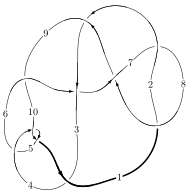
\includegraphics[width=112pt]{../../../GIT/diagram.site/Diagrams/png/128_10_44.png}\\
\ \ \ A knot diagram\footnotemark}&
\allowdisplaybreaks
\textbf{Linearized knot diagam} \\
\cline{2-2}
 &
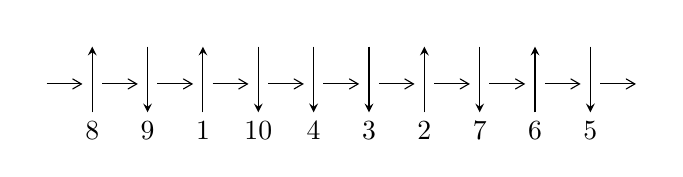
\begin{tikzpicture}[x=20pt, y=17pt]
	% nodes
	\node (C0) at (0, 0) {};
	\node (C1) at (1, 0) {};
	\node (C1U) at (1, +1) {};
	\node (C1D) at (1, -1) {8};

	\node (C2) at (2, 0) {};
	\node (C2U) at (2, +1) {};
	\node (C2D) at (2, -1) {9};

	\node (C3) at (3, 0) {};
	\node (C3U) at (3, +1) {};
	\node (C3D) at (3, -1) {1};

	\node (C4) at (4, 0) {};
	\node (C4U) at (4, +1) {};
	\node (C4D) at (4, -1) {10};

	\node (C5) at (5, 0) {};
	\node (C5U) at (5, +1) {};
	\node (C5D) at (5, -1) {4};

	\node (C6) at (6, 0) {};
	\node (C6U) at (6, +1) {};
	\node (C6D) at (6, -1) {3};

	\node (C7) at (7, 0) {};
	\node (C7U) at (7, +1) {};
	\node (C7D) at (7, -1) {2};

	\node (C8) at (8, 0) {};
	\node (C8U) at (8, +1) {};
	\node (C8D) at (8, -1) {7};

	\node (C9) at (9, 0) {};
	\node (C9U) at (9, +1) {};
	\node (C9D) at (9, -1) {6};

	\node (C10) at (10, 0) {};
	\node (C10U) at (10, +1) {};
	\node (C10D) at (10, -1) {5};
	\node (C11) at (11, 0) {};

	% arrows
	\draw[->,>={angle 60}]
	(C0) edge (C1) (C1) edge (C2) (C2) edge (C3) (C3) edge (C4) (C4) edge (C5) (C5) edge (C6) (C6) edge (C7) (C7) edge (C8) (C8) edge (C9) (C9) edge (C10) (C10) edge (C11) ;	\draw[->,>=stealth]
	(C1D) edge (C1U) (C2U) edge (C2D) (C3D) edge (C3U) (C4U) edge (C4D) (C5U) edge (C5D) (C6U) edge (C6D) (C7D) edge (C7U) (C8U) edge (C8D) (C9D) edge (C9U) (C10U) edge (C10D) ;
	\end{tikzpicture} \\
\hhline{~~} \\& 
\textbf{Solving Sequence} \\ \cline{2-2} 
 &
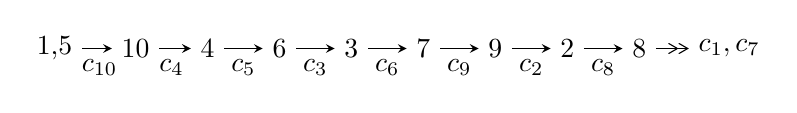
\begin{tikzpicture}[x=26pt, y=7pt]
	% node
	\node (A0) at (-1/8, 0) {1,5};
	\node (A1) at (1, 0) {10};
	\node (A2) at (2, 0) {4};
	\node (A3) at (3, 0) {6};
	\node (A4) at (4, 0) {3};
	\node (A5) at (5, 0) {7};
	\node (A6) at (6, 0) {9};
	\node (A7) at (7, 0) {2};
	\node (A8) at (8, 0) {8};
	\node (C1) at (1/2, -1) {$c_{10}$};
	\node (C2) at (3/2, -1) {$c_{4}$};
	\node (C3) at (5/2, -1) {$c_{5}$};
	\node (C4) at (7/2, -1) {$c_{3}$};
	\node (C5) at (9/2, -1) {$c_{6}$};
	\node (C6) at (11/2, -1) {$c_{9}$};
	\node (C7) at (13/2, -1) {$c_{2}$};
	\node (C8) at (15/2, -1) {$c_{8}$};
	\node (A9) at (37/4, 0) {$c_{1},c_{7}$};

	% edge
	\draw[->,>=stealth]	
	(A0) edge (A1) (A1) edge (A2) (A2) edge (A3) (A3) edge (A4) (A4) edge (A5) (A5) edge (A6) (A6) edge (A7) (A7) edge (A8) ;
	\draw[->>,>={angle 60}]	
	(A8) edge (A9);
\end{tikzpicture} \\ 

\end{tabular} \\

\footnotetext{
The image of knot diagram is generated by the software ``\textbf{Draw programme}" developed by Andrew Bartholomew(\url{http://www.layer8.co.uk/maths/draw/index.htm\#Running-draw}), where we modified some parts for our purpose(\url{https://github.com/CATsTAILs/LinksPainter}).
}\phantom \\ \newline 
\centering \textbf{Ideals for irreducible components\footnotemark of $X_{\text{par}}$} 
 
\begin{align*}
I^u_{1}&=\langle 
u^{39}- u^{38}+\cdots+2 u-1\rangle \\
\\
\end{align*}
\raggedright * 1 irreducible components of $\dim_{\mathbb{C}}=0$, with total 39 representations.\\
\footnotetext{All coefficients of polynomials are rational numbers. But the coefficients are sometimes approximated in decimal forms when there is not enough margin.}
\newpage
\renewcommand{\arraystretch}{1}
\centering \section*{I. $I^u_{1}= \langle u^{39}- u^{38}+\cdots+2 u-1 \rangle$}
\flushleft \textbf{(i) Arc colorings}\\
\begin{tabular}{m{7pt} m{180pt} m{7pt} m{180pt} }
\flushright $a_{1}=$&$\begin{pmatrix}1\\0\end{pmatrix}$ \\
\flushright $a_{5}=$&$\begin{pmatrix}0\\u\end{pmatrix}$ \\
\flushright $a_{10}=$&$\begin{pmatrix}1\\- u^2\end{pmatrix}$ \\
\flushright $a_{4}=$&$\begin{pmatrix}u\\- u^3+u\end{pmatrix}$ \\
\flushright $a_{6}=$&$\begin{pmatrix}- u^3\\u^5- u^3+u\end{pmatrix}$ \\
\flushright $a_{3}=$&$\begin{pmatrix}u^3\\- u^3+u\end{pmatrix}$ \\
\flushright $a_{7}=$&$\begin{pmatrix}- u^{11}+2 u^9-2 u^7- u^3\\u^{11}-3 u^9+4 u^7- u^5- u^3+u\end{pmatrix}$ \\
\flushright $a_{9}=$&$\begin{pmatrix}u^6- u^4+1\\- u^8+2 u^6-2 u^4\end{pmatrix}$ \\
\flushright $a_{2}=$&$\begin{pmatrix}u^{17}-4 u^{15}+7 u^{13}-4 u^{11}-3 u^9+6 u^7-2 u^5+u\\- u^{19}+5 u^{17}-12 u^{15}+15 u^{13}-9 u^{11}- u^9+4 u^7-2 u^5- u^3+u\end{pmatrix}$ \\
\flushright $a_{8}=$&$\begin{pmatrix}- u^{30}+7 u^{28}+\cdots-2 u^{12}+1\\u^{30}-8 u^{28}+\cdots+4 u^6- u^2\end{pmatrix}$\\&\end{tabular}
\flushleft \textbf{(ii) Obstruction class $= -1$}\\~\\
\flushleft \textbf{(iii) Cusp Shapes $= -4 u^{38}+44 u^{36}-4 u^{35}-232 u^{34}+40 u^{33}+752 u^{32}-192 u^{31}-1620 u^{30}+564 u^{29}+2316 u^{28}-1092 u^{27}-1948 u^{26}+1380 u^{25}+284 u^{24}-980 u^{23}+1508 u^{22}+16 u^{21}-1892 u^{20}+728 u^{19}+776 u^{18}-660 u^{17}+444 u^{16}+64 u^{15}-692 u^{14}+332 u^{13}+236 u^{12}-252 u^{11}+128 u^{10}-4 u^9-132 u^8+96 u^7+20 u^6-40 u^5+20 u^4-8 u^3-8 u^2+12 u-10$}\\~\\
\newpage\renewcommand{\arraystretch}{1}
\flushleft \textbf{(iv) u-Polynomials at the component}\newline \\
\begin{tabular}{m{50pt}|m{274pt}}
Crossings & \hspace{64pt}u-Polynomials at each crossing \\
\hline $$\begin{aligned}c_{1},c_{7}\end{aligned}$$&$\begin{aligned}
&u^{39}- u^{38}+\cdots+2 u^3+1
\end{aligned}$\\
\hline $$\begin{aligned}c_{2}\end{aligned}$$&$\begin{aligned}
&u^{39}+u^{38}+\cdots-18 u+17
\end{aligned}$\\
\hline $$\begin{aligned}c_{3},c_{9}\end{aligned}$$&$\begin{aligned}
&u^{39}+3 u^{38}+\cdots+12 u+1
\end{aligned}$\\
\hline $$\begin{aligned}c_{4},c_{10}\end{aligned}$$&$\begin{aligned}
&u^{39}+u^{38}+\cdots+2 u+1
\end{aligned}$\\
\hline $$\begin{aligned}c_{5}\end{aligned}$$&$\begin{aligned}
&u^{39}+21 u^{38}+\cdots-2 u^2+1
\end{aligned}$\\
\hline $$\begin{aligned}c_{6}\end{aligned}$$&$\begin{aligned}
&u^{39}-5 u^{38}+\cdots-12 u+1
\end{aligned}$\\
\hline $$\begin{aligned}c_{8}\end{aligned}$$&$\begin{aligned}
&u^{39}+19 u^{38}+\cdots+2 u^2-1
\end{aligned}$\\
\hline
\end{tabular}\\~\\
\newpage\renewcommand{\arraystretch}{1}
\flushleft \textbf{(v) Riley Polynomials at the component}\newline \\
\begin{tabular}{m{50pt}|m{274pt}}
Crossings & \hspace{64pt}Riley Polynomials at each crossing \\
\hline $$\begin{aligned}c_{1},c_{7}\end{aligned}$$&$\begin{aligned}
&y^{39}+19 y^{38}+\cdots+2 y^2-1
\end{aligned}$\\
\hline $$\begin{aligned}c_{2}\end{aligned}$$&$\begin{aligned}
&y^{39}-13 y^{38}+\cdots+3588 y-289
\end{aligned}$\\
\hline $$\begin{aligned}c_{3},c_{9}\end{aligned}$$&$\begin{aligned}
&y^{39}+31 y^{38}+\cdots-36 y-1
\end{aligned}$\\
\hline $$\begin{aligned}c_{4},c_{10}\end{aligned}$$&$\begin{aligned}
&y^{39}-21 y^{38}+\cdots+2 y^2-1
\end{aligned}$\\
\hline $$\begin{aligned}c_{5}\end{aligned}$$&$\begin{aligned}
&y^{39}-5 y^{38}+\cdots+4 y-1
\end{aligned}$\\
\hline $$\begin{aligned}c_{6}\end{aligned}$$&$\begin{aligned}
&y^{39}- y^{38}+\cdots+28 y-1
\end{aligned}$\\
\hline $$\begin{aligned}c_{8}\end{aligned}$$&$\begin{aligned}
&y^{39}+3 y^{38}+\cdots+4 y-1
\end{aligned}$\\
\hline
\end{tabular}\\~\\
\newpage\flushleft \textbf{(vi) Complex Volumes and Cusp Shapes}
$$\begin{array}{c|c|c}  
\text{Solutions to }I^u_{1}& \I (\text{vol} + \sqrt{-1}CS) & \text{Cusp shape}\\
 \hline 
\begin{aligned}
u &= \phantom{-}0.913577 + 0.379498 I\end{aligned}
 & -2.06381 - 1.25772 I & -6.67108 + 2.89583 I \\ \hline\begin{aligned}
u &= \phantom{-}0.913577 - 0.379498 I\end{aligned}
 & -2.06381 + 1.25772 I & -6.67108 - 2.89583 I \\ \hline\begin{aligned}
u &= \phantom{-}0.867921 + 0.539600 I\end{aligned}
 & -0.02772 - 7.71489 I & -1.96279 + 8.94046 I \\ \hline\begin{aligned}
u &= \phantom{-}0.867921 - 0.539600 I\end{aligned}
 & -0.02772 + 7.71489 I & -1.96279 - 8.94046 I \\ \hline\begin{aligned}
u &= -0.824609 + 0.517095 I\end{aligned}
 & \phantom{-}1.91036 + 2.98443 I & \phantom{-}1.85991 - 4.48194 I \\ \hline\begin{aligned}
u &= -0.824609 - 0.517095 I\end{aligned}
 & \phantom{-}1.91036 - 2.98443 I & \phantom{-}1.85991 + 4.48194 I \\ \hline\begin{aligned}
u &= -1.027710 + 0.074094 I\end{aligned}
 & -4.16770 + 3.61917 I & -10.06501 - 4.33455 I \\ \hline\begin{aligned}
u &= -1.027710 - 0.074094 I\end{aligned}
 & -4.16770 - 3.61917 I & -10.06501 + 4.33455 I \\ \hline\begin{aligned}
u &= \phantom{-}0.898181\phantom{ +0.000000I}\end{aligned}
 & -1.46294\phantom{ +0.000000I} & -6.39810\phantom{ +0.000000I} \\ \hline\begin{aligned}
u &= -0.704254 + 0.512490 I\end{aligned}
 & \phantom{-}2.25704 + 1.23434 I & \phantom{-}3.23691 - 3.43750 I \\ \hline\begin{aligned}
u &= -0.704254 - 0.512490 I\end{aligned}
 & \phantom{-}2.25704 - 1.23434 I & \phantom{-}3.23691 + 3.43750 I \\ \hline\begin{aligned}
u &= \phantom{-}0.632327 + 0.547010 I\end{aligned}
 & \phantom{-}0.63380 + 3.33294 I & \phantom{-}0.02170 - 2.50936 I \\ \hline\begin{aligned}
u &= \phantom{-}0.632327 - 0.547010 I\end{aligned}
 & \phantom{-}0.63380 - 3.33294 I & \phantom{-}0.02170 + 2.50936 I \\ \hline\begin{aligned}
u &= \phantom{-}0.139221 + 0.807285 I\end{aligned}
 & -3.46412 + 8.12134 I & -3.90397 - 6.02892 I \\ \hline\begin{aligned}
u &= \phantom{-}0.139221 - 0.807285 I\end{aligned}
 & -3.46412 - 8.12134 I & -3.90397 + 6.02892 I \\ \hline\begin{aligned}
u &= \phantom{-}1.114960 + 0.441427 I\end{aligned}
 & -2.49096 - 1.59434 I & -3.82288 + 0.43137 I \\ \hline\begin{aligned}
u &= \phantom{-}1.114960 - 0.441427 I\end{aligned}
 & -2.49096 + 1.59434 I & -3.82288 - 0.43137 I \\ \hline\begin{aligned}
u &= \phantom{-}0.076025 + 0.793162 I\end{aligned}
 & -5.24072 + 0.25023 I & -6.76221 + 0.26522 I \\ \hline\begin{aligned}
u &= \phantom{-}0.076025 - 0.793162 I\end{aligned}
 & -5.24072 - 0.25023 I & -6.76221 - 0.26522 I \\ \hline\begin{aligned}
u &= -0.132738 + 0.775160 I\end{aligned}
 & -1.00162 - 3.25758 I & -0.69216 + 2.50620 I \\ \hline\begin{aligned}
u &= -0.132738 - 0.775160 I\end{aligned}
 & -1.00162 + 3.25758 I & -0.69216 - 2.50620 I \\ \hline\begin{aligned}
u &= -1.142370 + 0.483180 I\end{aligned}
 & -2.09760 + 6.17588 I & -2.65093 - 6.87938 I \\ \hline\begin{aligned}
u &= -1.142370 - 0.483180 I\end{aligned}
 & -2.09760 - 6.17588 I & -2.65093 + 6.87938 I \\ \hline\begin{aligned}
u &= \phantom{-}1.194180 + 0.388571 I\end{aligned}
 & -4.89443 - 0.66747 I & -5.40097 + 0.84813 I \\ \hline\begin{aligned}
u &= \phantom{-}1.194180 - 0.388571 I\end{aligned}
 & -4.89443 + 0.66747 I & -5.40097 - 0.84813 I \\ \hline\begin{aligned}
u &= -1.213030 + 0.378072 I\end{aligned}
 & -7.52915 - 4.12434 I & -8.59821 + 2.83806 I \\ \hline\begin{aligned}
u &= -1.213030 - 0.378072 I\end{aligned}
 & -7.52915 + 4.12434 I & -8.59821 - 2.83806 I \\ \hline\begin{aligned}
u &= -1.210580 + 0.415258 I\end{aligned}
 & -9.04143 + 3.95701 I & -10.59268 - 3.75109 I \\ \hline\begin{aligned}
u &= -1.210580 - 0.415258 I\end{aligned}
 & -9.04143 - 3.95701 I & -10.59268 + 3.75109 I \\ \hline\begin{aligned}
u &= -1.185450 + 0.504016 I\end{aligned}
 & -4.07758 + 7.98510 I & -3.85690 - 5.54137 I\\
 \hline 
 \end{array}$$\newpage$$\begin{array}{c|c|c}  
\text{Solutions to }I^u_{1}& \I (\text{vol} + \sqrt{-1}CS) & \text{Cusp shape}\\
 \hline 
\begin{aligned}
u &= -1.185450 - 0.504016 I\end{aligned}
 & -4.07758 - 7.98510 I & -3.85690 + 5.54137 I \\ \hline\begin{aligned}
u &= \phantom{-}1.200000 + 0.486246 I\end{aligned}
 & -8.53633 - 4.91106 I & -9.80910 + 3.06121 I \\ \hline\begin{aligned}
u &= \phantom{-}1.200000 - 0.486246 I\end{aligned}
 & -8.53633 + 4.91106 I & -9.80910 - 3.06121 I \\ \hline\begin{aligned}
u &= \phantom{-}1.194900 + 0.512673 I\end{aligned}
 & -6.5788 - 12.9690 I & -6.91871 + 9.04784 I \\ \hline\begin{aligned}
u &= \phantom{-}1.194900 - 0.512673 I\end{aligned}
 & -6.5788 + 12.9690 I & -6.91871 - 9.04784 I \\ \hline\begin{aligned}
u &= -0.180542 + 0.637095 I\end{aligned}
 & \phantom{-}0.64272 - 1.83013 I & \phantom{-}1.22482 + 3.69155 I \\ \hline\begin{aligned}
u &= -0.180542 - 0.637095 I\end{aligned}
 & \phantom{-}0.64272 + 1.83013 I & \phantom{-}1.22482 - 3.69155 I \\ \hline\begin{aligned}
u &= \phantom{-}0.339086 + 0.540694 I\end{aligned}
 & -0.25067 - 2.27932 I & -0.43670 + 3.34383 I \\ \hline\begin{aligned}
u &= \phantom{-}0.339086 - 0.540694 I\end{aligned}
 & -0.25067 + 2.27932 I & -0.43670 - 3.34383 I\\
 \hline 
 \end{array}$$\newpage
\newpage\renewcommand{\arraystretch}{1}
\centering \section*{ II. u-Polynomials}
\begin{tabular}{m{50pt}|m{274pt}}
Crossings & \hspace{64pt}u-Polynomials at each crossing \\
\hline $$\begin{aligned}c_{1},c_{7}\end{aligned}$$&$\begin{aligned}
&u^{39}- u^{38}+\cdots+2 u^3+1
\end{aligned}$\\
\hline $$\begin{aligned}c_{2}\end{aligned}$$&$\begin{aligned}
&u^{39}+u^{38}+\cdots-18 u+17
\end{aligned}$\\
\hline $$\begin{aligned}c_{3},c_{9}\end{aligned}$$&$\begin{aligned}
&u^{39}+3 u^{38}+\cdots+12 u+1
\end{aligned}$\\
\hline $$\begin{aligned}c_{4},c_{10}\end{aligned}$$&$\begin{aligned}
&u^{39}+u^{38}+\cdots+2 u+1
\end{aligned}$\\
\hline $$\begin{aligned}c_{5}\end{aligned}$$&$\begin{aligned}
&u^{39}+21 u^{38}+\cdots-2 u^2+1
\end{aligned}$\\
\hline $$\begin{aligned}c_{6}\end{aligned}$$&$\begin{aligned}
&u^{39}-5 u^{38}+\cdots-12 u+1
\end{aligned}$\\
\hline $$\begin{aligned}c_{8}\end{aligned}$$&$\begin{aligned}
&u^{39}+19 u^{38}+\cdots+2 u^2-1
\end{aligned}$\\
\hline
\end{tabular}\newpage\renewcommand{\arraystretch}{1}
\centering \section*{ III. Riley Polynomials}
\begin{tabular}{m{50pt}|m{274pt}}
Crossings & \hspace{64pt}Riley Polynomials at each crossing \\
\hline $$\begin{aligned}c_{1},c_{7}\end{aligned}$$&$\begin{aligned}
&y^{39}+19 y^{38}+\cdots+2 y^2-1
\end{aligned}$\\
\hline $$\begin{aligned}c_{2}\end{aligned}$$&$\begin{aligned}
&y^{39}-13 y^{38}+\cdots+3588 y-289
\end{aligned}$\\
\hline $$\begin{aligned}c_{3},c_{9}\end{aligned}$$&$\begin{aligned}
&y^{39}+31 y^{38}+\cdots-36 y-1
\end{aligned}$\\
\hline $$\begin{aligned}c_{4},c_{10}\end{aligned}$$&$\begin{aligned}
&y^{39}-21 y^{38}+\cdots+2 y^2-1
\end{aligned}$\\
\hline $$\begin{aligned}c_{5}\end{aligned}$$&$\begin{aligned}
&y^{39}-5 y^{38}+\cdots+4 y-1
\end{aligned}$\\
\hline $$\begin{aligned}c_{6}\end{aligned}$$&$\begin{aligned}
&y^{39}- y^{38}+\cdots+28 y-1
\end{aligned}$\\
\hline $$\begin{aligned}c_{8}\end{aligned}$$&$\begin{aligned}
&y^{39}+3 y^{38}+\cdots+4 y-1
\end{aligned}$\\
\hline
\end{tabular}
\vskip 2pc
\end{document}